\section{Plotting}
This section talks about how to utilize the plotting function provided by pbdPROF.You just need to run the code in 

\subsection{Plotting of fpmpi library for pbdMPI codes}
Plotting can utilized in two ways:
\begin{enumerate}
\item For plotting just run your code in R console similar to below 
\begin{Code}
source("allreduce.r")
\end{Code}
\item If you are using Rscript command and you have the fpmpi profiling library text output.
You have code do similar to below in R console
\begin{Code}
x<-read.prof("profiled_text_file.txt")
plot(x)
\end{Code}
\end{enumerate}
here you have made an object of the parsing output and used that in plot function.

\begin{figure}%                 use [hb] only if necceccary!
  \centering
  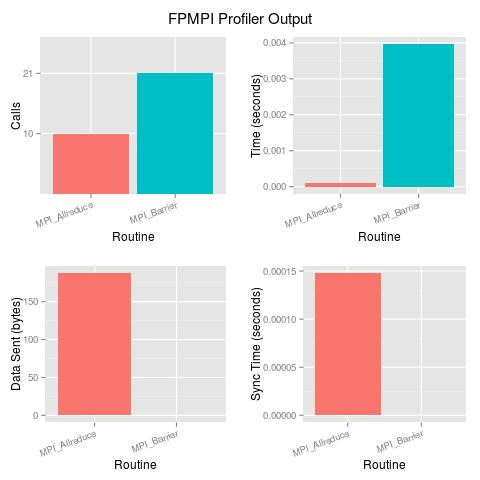
\includegraphics[width=10cm]{./include/fpmpi_pbdMPI_plot.jpeg}
  \caption{plot figure}
  \label{fig:plot_fpmpi}

\end{figure}


\subsection{Plotting of fpmpi library for Rmpi codes}
Plotting can utilized in two ways:
\begin{enumerate}
\item For plotting just run your code in R console similar to below 
\begin{Code}
source("masterslavePI.r")
\end{Code}
\item If you are using Rscript command and you have the fpmpi profiling library text output.
You have code do similar to below in R console
\begin{Code}
x<-read.prof("profiled_text_file.txt")
plot(x)
\end{Code}
here you have made an object of the parsing output and used that in plot function.
\end{enumerate}





